\documentclass[14pt]{extarticle}

\usepackage[utf8]{inputenc}
\usepackage[english,ukrainian]{babel}
\usepackage{bookmark}
\usepackage{libertine}

\usepackage{amsmath,amssymb}
\usepackage{parskip}
\usepackage{graphicx}
\usepackage[table]{xcolor}
\usepackage{tcolorbox}
\tcbuselibrary{skins}
\usepackage[framemethod=tikz]{mdframed}
\usepackage{chngcntr}
\usepackage{enumitem}
\usepackage{hyperref}
\usepackage{float}
\usepackage{subfig}
\usepackage{chngcntr}
\usepackage{esint}
\usepackage{pdfpages} % Add this to your preamble

\usepackage{libertinus}
\renewcommand\ttdefault{cmtt}

\usepackage[top=2.5cm, left=3cm, right=3cm, bottom=4.0cm]{geometry}
\usepackage{algorithm}
\usepackage{algpseudocode}
\usepackage{listings}
\usepackage{xcolor}

\usepackage[cache=false]{minted}
\usemintedstyle{tango}

\definecolor{codegreen}{rgb}{0,0.6,0}
\definecolor{codegray}{rgb}{0.5,0.5,0.5}
\definecolor{codepurple}{rgb}{0.58,0,0.82}
\definecolor{backcolour}{rgb}{0.95,0.95,0.92}

\lstdefinestyle{mystyle}{
    backgroundcolor=\color{backcolour},   
    commentstyle=\color{codegreen},
    keywordstyle=\color{magenta},
    numberstyle=\tiny\color{codegray},
    stringstyle=\color{codepurple},
    basicstyle=\ttfamily\footnotesize,
    breakatwhitespace=false,         
    breaklines=true,                 
    captionpos=b,                    
    keepspaces=true,                 
    numbers=left,                    
    numbersep=5pt,                  
    showspaces=false,                
    showstringspaces=false,
    showtabs=false,                  
    tabsize=2
}
\lstset{style=mystyle}

\usepackage{ragged2e}
\begin{document}

\begin{titlepage}
	\centering
	%
\includegraphics[width=0.15\textwidth]{images/lab_1/logo.png}\par\vspace{0.3cm}
	{\textbf{Міністерство освіти і науки України}\par
 Харківський національний університет імені В.Н. Каразіна\par}
    \vspace{1cm}
	{\Large \textsc{Розрахунково-графічне завдання \#4}\par
    \textbf{Чисельне розв'язання інтегральних рівнянь}\par}
	\vfill
 \begin{FlushRight}
	\textbf{Виконав:}\par Захаров Дмитро Олегович \par Група МП-41
\end{FlushRight}
	\vfill

% Bottom of the page
	{\large Харків -- 2025\par}
\end{titlepage}

\tableofcontents
\pagebreak

\section{Постановка задачі}

Розв'язати методом квадратур інтегральне рівняння
\begin{equation*}
    y(x) - \int_0^1 \cos (0.5 xt)y(t)dt = \sqrt{1+x^2}
\end{equation*}

\section{Опис методів}

\subsection{Метод квадратур}

Нехай ми маємо інтегральне рівняння Фредгольма 2-го роду
\begin{equation*}
    y(x) = \lambda\int_a^b K(x,t)y(t)dt + f(x), \quad x \in [a,b],
\end{equation*}

Метод квадратур полягає у заміні визначеного інтегралу $\int_a^b F(x)dx$ на суму
$\sum_{i=1}^n A_iF(x_i) + R(F)$, де $R(F)$ --- мала нев'язка. Таким чином,
розіб'ємо відрізок $[a,b]$ на $n$ частин таким чином, що $x_i=a+(i-1)h$ для
$h=\frac{b-a}{n-1}$, та позначимо $y_i := y(x_i)$, $f_i := f(x_i)$, $K_{i,j} :=
K(x_i,x_j)$. Тоді, використовуючи заміну, маємо:
\begin{equation*}
    y_i = f_i + \lambda \sum_{j=1}^n A_jK_{i,j}y_j + R_i.
\end{equation*}

Відкинувши $R_i$ та позначивши $v_i \approx y(x_i)$ --- наближене значення $y$
у точці $x_i$, отримаємо систему лінійних алгебраїчних рівнянь
\begin{equation*}
    v_i = f_i + \lambda \sum_{j=1}^n A_jK_{i,j}v_j, \quad i=1,\ldots,n.
\end{equation*}

Коли ми знайдемо $v_i$, то зможемо знайти наближений розв'язок $\widehat{y}$ за
формулою
\begin{equation*}
    \widehat{y}(x) = f(x) + \lambda\sum_{j=1}^n A_jK(x,x_j)v_j.
\end{equation*}

\section{Імплементація}

\subsection{Методологія}

В нашому прикладі маємо:
\begin{equation*}
    f(x) = \sqrt{1+x^2}, \quad K(x,t) = \cos(0.5xt), \quad a=0, \quad b=1.
\end{equation*}

Розділяємо відрізок на $n$ частин, отримуючи $x_i = ih$ для $h=\frac{1}{n}$.
Скористаємось формулою трапецій. Тоді, $A_1=A_n=\frac{1}{2}h$ і $A_j=h$ для всіх
інших $j$. Таким чином, можемо знайти наближене значення $y(x)$ в точках 
$x_i$ за допомогою системи лінійних алгебраїчних рівнянь
\begin{equation*}
    v_i = \sqrt{1+h^2i^2} + h\sum_{j=1}^n k_j \cos(0.5h^2ij) v_j, \quad k_j = \begin{cases}
        \frac{1}{2}, & j \in \{1,n\}, \\
        1, & j \not\in \{1,n\}.
    \end{cases}
\end{equation*}

\subsection{Код на Python}

Наступний код розв'язує зазане інтегральне рівняння методом квадратур:
\begin{minted}{python}
from typing import Callable

# Some math-related imports
import numpy as np
from scipy.sparse import lil_matrix
from scipy.sparse.linalg import spsolve


def solve_fredholm(
    n: int, 
    a: float, 
    b: float, 
    kernel: Callable[[np.ndarray, np.ndarray], np.ndarray],
    f_func: Callable[[np.ndarray], np.ndarray],
) -> Callable[[np.ndarray], np.ndarray]:
    """
    Solves the Fredholm integral equation of the second kind:
    """
    
def solve_fredholm(
    n: int, 
    a: float, 
    b: float, 
    kernel: Callable[[np.ndarray, np.ndarray], np.ndarray],
    f_func: Callable[[np.ndarray], np.ndarray],
) -> Callable[[np.ndarray], np.ndarray]:
    """
    Solves the Fredholm integral equation of the second kind:
    """
    
    h = (b - a) / n  # Step size
    xs = np.linspace(a, b, n+1)  # Grid points
    
    weights = h * np.ones(n+1)  # Coefficients for the integral trapezoid approximation
    weights[0] = weights[n] = 0.5 * h # Trapezoidal rule for endpoints
    
    b = np.zeros(n+1) # Initialize the solution vector
    M = np.zeros((n+1, n+1)) # Coefficient matrix
    
    # Now, we fill the matrix A and the vector v
    for i in range(n+1):
        b[i] = f_func(xs[i]) # Free term is easy to compute
        
        for j in range(n+1):
            delta = 1.0 if i == j else 0.0
            M[i,j] = delta - kernel(xs[i], xs[j]) * weights[j]

    v = np.linalg.solve(M, b) # Solve the linear system
    
    def resultant_fn(x: np.ndarray) -> np.ndarray:
        """
        Returns the resultant function y(x).
        """
    
        return f_func(x) + np.sum(weights * kernel(xs, x) * v)
    
    return resultant_fn
\end{minted}

Наступний код виконує розв'язок інтегрального рівняння, заданого вище:
\begin{minted}{python}
import numpy as np
import matplotlib.pyplot as plt

from solver import solve_fredholm

if __name__ == "__main__":
    # Problem parameters
    a, b = 0.0, 1.0
    n = 20 # Number of grid points
    f_func = lambda x: np.sqrt(1 + x**2)
    kernel = lambda x, y: np.cos(0.5 * x * y)
    
    # Solve the Fredholm integral equation
    y_solution = solve_fredholm(n, a, b, kernel, f_func)
    
    # Plot the solution
    x_vals = np.linspace(a, b, n)
    y_vals = np.array([y_solution(x_vals[i]) for i in range(n)], dtype=np.float64)
    
    plt.plot(x_vals, y_vals, label="Numerical Solution", color='blue', linewidth=3)
    plt.title("Solution to the Fredholm Integral Equation")
    plt.xlabel("x")
    plt.ylabel("y(x)")
    plt.legend()
    plt.grid()
    plt.savefig("fredholm_solution.pdf", dpi=300)
    plt.show()
\end{minted}

Результат зображено на Рисунку \ref{fig:fredholm_solution}.

\begin{figure}[H]
    \centering
    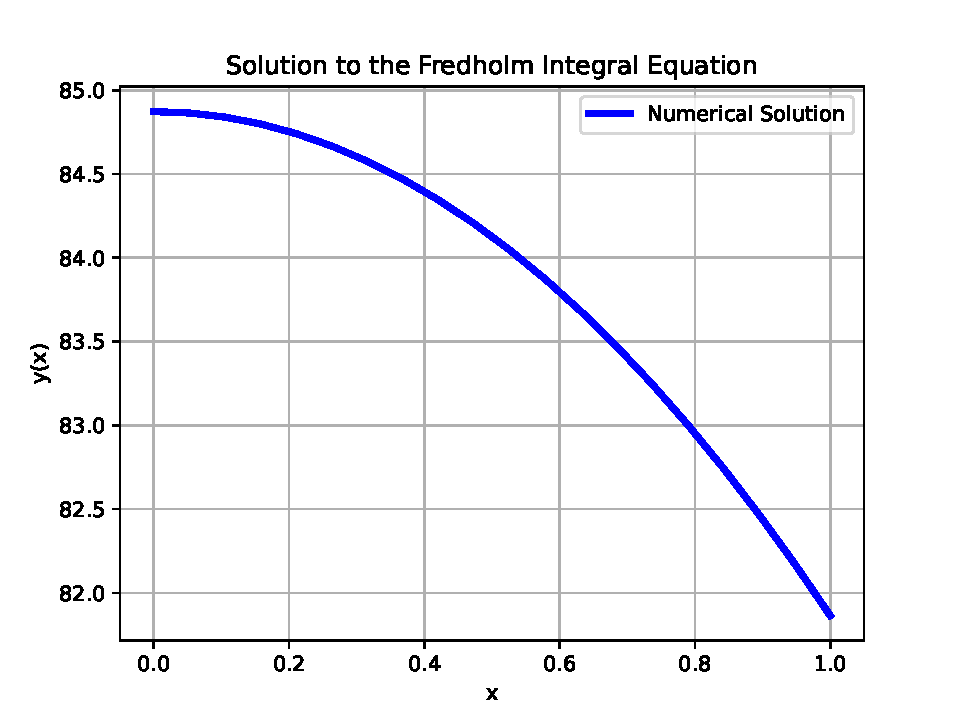
\includegraphics[width=\textwidth]{appendices/homework_4/fredholm_solution.pdf}
    \caption{Графік розв'язку інтегрального рівняння Фредгольма 2-го роду для 
    $n=20$}
    \label{fig:fredholm_solution}
\end{figure}

\end{document}

